\documentclass{article}
\usepackage{amsmath}
\usepackage{amssymb}
\usepackage{listings}
\usepackage{graphicx}
\usepackage{hyperref}
\usepackage{listings}
\usepackage{xcolor}
\usepackage{amsmath}
\usepackage[T1]{fontenc}
\usepackage[brazil]{babel}
\usepackage{mathrsfs}
\definecolor{codegreen}{rgb}{0,0.6,0}
\definecolor{codegray}{rgb}{0.5,0.5,0.5}
\definecolor{codepurple}{rgb}{0.8,0,0.2}
\definecolor{backcolour}{rgb}{.95,.95,1}

\lstset{
    basicstyle=\ttfamily\footnotesize,
    backgroundcolor=\color{backcolour},
    commentstyle=\color{codegreen},
    keywordstyle=\color{magenta},
    numberstyle=\tiny\color{codegray},
    stringstyle=\color{codepurple},
    inputencoding=utf8,
    extendedchars=true,
    breaklines=true,
    captionpos=b,
    keepspaces=true,
    numbers=left,
    numbersep=5pt,
    showspaces=false,
    showstringspaces=false,
    showtabs=false,
    tabsize=2,
    morecomment=[l]{//},
    morecomment=[s]{/*}{*/},
    morecomment=[s]{"""}{"""}
}


\title{Explicacão do Código Python para Criptografia RSA com OAEP e Base64}
\author{Davi de Araújo Garcez Bueno - 211060586 \\ Erick Hideki Taira - 222011525}
\date{Janeiro 2025}

\begin{document}

\maketitle

\section{Introdução}
Os códigos apresentados implementam um sistema de criptografia baseado no algoritmo RSA, combinando técnicas como o OAEP (Optimal Asymmetric Encryption Padding), 
 codificacão em Base64 e teste de primalidade de Miller-Rabin para identificar números primos. Além disso, ele realiza assinaturas digitais utilizando um esquema que
 utiliza o RSA e também é possível verifica a autenticidade da assinatura.

\section{Introdução Teórica}

O algoritmo RSA é um sistema de criptografia assimétrica que utiliza chaves públicas e privadas para a criptografia e descriptografia de mensagens.
A segurança do RSA é baseada na dificuldade de fatorar o produto de dois números primos grandes. Porém, o algoritmo RSA, sozinho, para uma mesma mensagem,
retorna sempre o mesmo texto criptografado. Isso torna o algoritmo suscetível a ataques de análise de frequência,
onde o atacante pode identificar padrões e inferir informações sobre a mensagem original.

Para mitigar essa vulnerabilidade, técnicas adicionais como o OAEP (Optimal Asymmetric Encryption Padding) são utilizadas.
O OAEP adiciona um preenchimento aleatório à mensagem antes da criptografia,
garantindo que textos iguais resultem em criptogramas diferentes.
Além disso, a codificação Base64 é empregada para converter dados binários em uma representação textual,
facilitando a manipulação e transmissão segura das mensagens.

Outro componente essencial do sistema é o teste de primalidade de Miller-Rabin, utilizado para garantir
 que os números gerados para as chaves sejam realmente primos. A assinatura digital com RSA também é
  implementada para assegurar a autenticidade e integridade das mensagens, permitindo que o receptor
   verifique se a mensagem foi enviada pelo remetente legítimo e não foi alterada durante a transmissão.

\section{Fluxo Geral da Implementação}

\begin{enumerate}
    \item Geração de dois números primos p e q.
    \subitem - Miller Rabin
    \subsubitem - Decompondo
    \subitem - Gerar Primos de 1024 bits
    \item Cálculo de n e de phi.
    \item Definição da chave pública e cálculo da chave privada.
    \item Codificação da mensagem em Base64, seguida do algoritmo OAEP.
    \item Criptografia da mensagem com RSA.
    \item Descriptografia da mensagem e reversão do processo de OAEP e Base64.
    \item Geração e verificação de uma assinatura digital.
    \item Teste de execução do programa.
    \item Impressão dos resultados.
\end{enumerate}

\section{Geração dos números primos}
\subsection*{Função \texttt{decompondo(n)}}
Esta funcão decompõe um número no seguinte formato. Ela será utilizada em uma das etapas do algoritmo 
de Miller Rabin.
\[
n = 2^ e \cdot m
\]

\begin{lstlisting}[language=Python]
def decompondo(n):
    # Decompoe n-1 como 2 elevado a e vezes m, onde n e impar.
    # Args:
    #    n: numero para decompor
    # Returns:
    #    int: expoente
    #    int: numero
        e = 0
        m = n - 1
        while m % 2 == 0:
            m //= 2        
            e += 1
        return e, m
\end{lstlisting}

\subsection{Função \texttt{miller\textunderscore rabin}}
Implementa o teste de primalidade de Miller-Rabin, retornando verdadeiro se o número for provavelmente primo e falso caso contrário.

\begin{lstlisting}[language=Python]
    def miller_rabin(n, rodadas=10):
    """
    Miller-Rabin primality test
    Args:
        n: numero para ser testado
        rodadas: quantidade de rodadas a serem feitas
    Returns:
        bool: True se e primo, False se nao e primo
    """
        if n <= 1 or n == 4:
            return False
        if n <= 3:
            return True
        if n % 2 == 0:
            return False
        
        expo_k, m = decompondo(n)  #exponte K e m tal que n - 1 = 2^k * m
        for _ in range(rodadas):
            a = random.randrange(2, n - 2) # pega um numero aleatorio entre 2 e n-2
            """ x = a^m mod n """
            x = pow(a, m, n) 
            if x == 1 or x == n-1: # se x for 1 ou n-1, entao n e primo
                continue
            else:
                teste = False
                for _ in range(expo_k - 1): # para i de 0 ate k-1
                    """ x = x^2 mod n """ 
                    x = pow(x, 2, n)
                    if x == n-1:
                        teste = True
                        break
                if(teste):
                    continue
                else:
                    return False
        return True
    \end{lstlisting}

\subsubsection*{Teste de primalidade de Miller-Rabin}

\subsubsection*{Teoria do Teste de Primalidade de Miller-Rabin}

O teste de primalidade de Miller-Rabin é um algoritmo probabilístico utilizado para determinar se um número é primo. Ele é baseado no pequeno teorema de Fermat, que afirma que se \( p \) é um número primo e \( a \) é um inteiro tal que \( 1 \leq a < p \), então:

\[
a^{p-1} \equiv 1 \pmod{p}
\]

O teste de Miller-Rabin estende essa ideia, verificando se um número composto pode ser identificado por
meio de várias iterações de um teste baseado em exponenciação modular. O algoritmo funciona da seguinte forma:\\
1. \textbf{Decompor}: Decompõe \( n-1 \) na forma \( 2^k \cdot m \), onde \( m \) é ímpar.\\
2. \textbf{Escolha de Testes}: Escolhe um número aleatório \( a \) tal que \( 2 \leq a \leq n-2 \).\\
3. \textbf{Exponenciação Modular}: Calcula \( x = a^m \mod n \).\\
4. \textbf{Verificação Inicial}: Se \( x = 1 \) ou \( x = n-1 \), então \( n \) pode ser primo.\\
5. \textbf{Iterações}: Para \( k-1 \) iterações, calcula \( x = x^2 \mod n \). Se em qualquer iteração \( x = n-1 \), então \( n \) pode ser primo.\\
6. \textbf{Conclusão}: Se nenhuma das condições acima for satisfeita, \( n \) é composto.\\

O teste é repetido várias vezes com diferentes valores de \( a \) para aumentar a confiança no resultado. Se o número passar em todas as iterações, ele é considerado provavelmente primo.

\subsection{Função \texttt{prime\textunderscore numbers}}
Gera dois números primos utilizando o teste de Miller-Rabin.

\begin{lstlisting}[language=Python]
    def prime_numbers(): #descobre os numeros primos usando a funcao de Miller-Rabin
    """
    Descobrindo os numeros primos
    Args: none
    Returns:
        list: lista com os numeros primos
    """
        n = 1 << 1024
        contador = 0
        par_de_numeros_primos = []
        while True:
            if miller_rabin(n):
                par_de_numeros_primos.append(n)
                contador += 1
            if contador == 2:
                break
            n += 1
        return par_de_numeros_primos
    \end{lstlisting}

É uma maneira bem rudimentar de descobrir o par de números primos com mais de 1024 bits, mas é suficiente para a nossa aplicação.
 Porém é importante ressaltar que para aplicações
 reais, é necessário um método mais robusto para a geração dos números primos, pois no nosso caso sempre será gerado os mesmos números primos.

\section{Implementação do OAEP}

\subsection{Função \texttt{mgf1}}
Mascara uma entrada utilizando uma funcão de hash para gerar uma saida pseudoaleatória de comprimento específico.

\begin{lstlisting}[language=Python]
    def mgf1(seed: int, length: int, hash_func=hashlib.sha1) -> bytes: #mascara de geracao de funcao
        if length > (hash_func().digest_size * (2**32)): #tamanho da mascara 
            raise ValueError("mask too long")
        # Converte o tamanho de bits para bytes
        byte_length = (length + 7) // 8
        # Converte a seed para um tamanho fixo de bytes
        seed_bytes = seed.to_bytes((seed.bit_length() + 7) // 8, byteorder='big')
        T = b""
        counter = 0
        while len(T) < byte_length: # enquanto o tamanho de T for menor que o tamanho de bytes
            C = counter.to_bytes(4, byteorder='big')
            T += hash_func(seed_bytes + C).digest()
            counter += 1
        return T[:byte_length]
    \end{lstlisting}

Não criamos o código acima retiramos de uma implementaçaõ encontrada na web.
O link estará disponibilizado nas referências.

\vspace{7 cm}
\subsection{Funções básicas}

\texttt{Shift\_left} e \texttt{Shift\_right} realizam o deslocamento dos bits para a esquerda e direita, respectivamente.
\texttt{MSB} calcula o bit mais significativo de um número. \texttt{Number\_of\_bits} calcula o número de bits de um número.

\begin{lstlisting}[language=Python]
    def shift_left(shift_values, n): #deslocamento para a esquerda
    """
    Shift Left
    Args:
        shift_values: quantidade de shift
        n: numero para ser shiftado
    Returns:
        int: numero shiftado
    """
        return n << shift_values

    def shift_right(shift_values, n): #deslocamento para a direita
    """
    Shift Right
    Args:
        shift_values: quantidade de shift
        n: numero para ser shiftado
    Returns:
        int: numero shiftado
    """
        return n >> shift_values

    def msb(n): #bit mais significativo
    """
    Most Significant Bit
    Args:
        n: numero para ser calculado o MSB
    Returns:
        int: MSB
    """
        msb = 0
        while n > 0:
            n >>= 1
            msb += 1
        return msb

    def number_of_bits(n): #calcula o numero de bits de um certo numero
    """
    Number of Bits
    Args:
        n: numero para ser calculado a quantidade de bits
    Returns:
        int: quantidade de bits
    """
        temp = n
        count = 0
        while(temp != 0):
            temp = shift_right(1, temp)
            count += 1
        return count


    \end{lstlisting}

\subsection{Função \texttt{DB}}
Concatena um hash  e uma mensagem, adicionando um preenchimento de no minimo 8 bits.

\begin{lstlisting}[language=Python]
    def DB(pHash, mensagem): #faz a concatenacao de pHash e mensagem
    """
    DB
    Obs:
        padding minimo de 8 bits
    Args:
        pHash: pHash
        mensagem: mensagem
    Returns:
        int: DB com padding
    """
        pHash = shift_left(1536 , pHash)
        padding = shift_left(number_of_bits(mensagem), 1)
        pHash = pHash | padding
        return (pHash | mensagem)
    \end{lstlisting}

    A função \texttt{DB} é responsável por concatenar um hash e uma mensagem, adicionando um preenchimento de no mínimo 8 bits, padding.
     O preenchimento é necessário para garantir que a mensagem tenha um comprimento adequado para o processo de criptografia.
      A função realiza as seguintes etapas:

    \begin{enumerate}
        \item Calcula o hash de um parámetro pré-definido (neste caso, \texttt{pHash(NULL)}).
        \item Desloca o hash para a esquerda em 1536 bits. Isso é necessário, pois o pHash deve ficar encaixado nos 256 bits mais significativos do DB.
        \item Calcula o padding necessário para a mensagem, setando em 1 o bit à esquerda do MSB da mensagem.
        \item Realiza a operação lógica OR com o pHash e o padding.
        \item Realiza a operação lógica OR com o resultado anterior e a mensagem.
    \end{enumerate}

    A função retorna o valor concatenado de 1792 bits, que será utilizado nas etapas subsequentes do processo de encapsulamento OAEP.

\vspace{4 cm}

\subsection{Função \texttt{enc\textunderscore oaep}}
Implementa a etapa de encapsulamento OAEP para preparacão da mensagem antes da criptografia RSA.

\begin{lstlisting}[language=Python]
    def enc_oaep(mensagem): #encriptacao OAEP
    """
    Encapsulamento OAEP
    Args:
        mensagem: mensagem
    Returns:
        int: EM
    """
        seed = random.getrandbits(256).to_bytes(32, byteorder="big")                                # gera uma seed aleatoria
        seed = int.from_bytes(seed, byteorder='big')                                                # converte a seed para int
        pHash = hashlib.sha3_256().digest()                                                         # hash de NULL
        pHash = int.from_bytes(pHash, byteorder='big')                                              # converte o hash da seed para int
        maskedDB = DB(pHash, mensagem) ^ int.from_bytes(mgf1(seed, 1792, hashlib.sha3_256))         # faz a concatenacao de pHash e mensagem
        maskedSeed = seed ^ int.from_bytes(mgf1(maskedDB, 32, hashlib.sha3_256))                    # faz a mascara da seed
        maskedSeed = shift_left(1792, maskedSeed)                                                   # desloca a seed para a esquerda em 1792 bits
        EM = maskedSeed | maskedDB                                                                  # concatena a mascara da seed e a mascara da mensagem
        return EM
    \end{lstlisting}

    \begin{enumerate}
        \item Geração da Seed: Uma seed aleatória de 256 bits é gerada e convertida para um inteiro.
        \item pHash de NULL: Um hash SHA-3 de 256 bits de NULL é gerado e convertido para um inteiro.
        \item maskedDB: A função \texttt{DB} concatena a \texttt{seed} com o \texttt{pHash} e realiza um \texttt(XOR)
         com a máscara gerada pela função \texttt{mgf1} na seed.
        \item maskedSeed: A MaskedSeed é criada pela seed \texttt{XOR} com a máscara gerada pela função \texttt{mgf1} no \texttt{maskedDB}.
        \item Deslocamento da maskedSeed: A maskedSeed é deslocada para a esquerda em 1792 bits.
        \item Concatenação Final: A maskedSeed é concatenada com um \texttt{OR} com o \texttt{maskedDB}.
    \end{enumerate}

\subsection{Função \texttt{dec\textunderscore oaep}}
Realiza a decodificacão OAEP para recuperar a mensagem original após a descriptografia RSA.

\begin{lstlisting}[language=Python]
    def dec_oaep(c): #decriptacao OAEP
    """
    Decriptando OAEP
    Args:
        c: EM
    Returns:
        int: m
    """
        bitMask = shift_left(1792, 1) - 1                                                           # mascara de bits
        maskedDB = c & bitMask
        maskedSeed = shift_right(1792, c)                                                                      # mascara de DB
        seed = maskedSeed ^ int.from_bytes(mgf1(maskedDB, 32, hashlib.sha3_256), byteorder='big')   #
        db = maskedDB ^ int.from_bytes(mgf1(seed, 1792, hashlib.sha3_256), byteorder='big')         #      
        bitMask = shift_left(1536, 1) - 1                                                           #
        m = db & bitMask                                                                            #
        MSBit = msb(m) - 1                                                                          #
        MSBit = shift_left(MSBit, 1)                                                                #
        m = m ^ MSBit                                                                               #
        return m
    \end{lstlisting}
    
    \begin{enumerate}
        \item Geração da Máscara de Bits:
        Uma máscara de bits é criada para isolar os últimos 1792 bits de \( c \). A função \texttt{shift\_left(1792, 1)} desloca o número 1 para a esquerda em 1792 bits, resultando em um número com 1792 zeros seguidos de um 1. Subtraindo 1, obtemos uma máscara com 1792 uns.
    
        \item Extraindo \texttt{maskedDB}:
        A operação \( \& \) (AND bit a bit) é usada para extrair os últimos 1792 bits de \( c \), que correspondem ao \texttt{maskedDB}.
    
        \item Extraindo \texttt{maskedSeed}:
        A função \texttt{shift\_right(1792, c)} desloca \( c \) para a direita em 1792 bits, isolando assim a \texttt{maskedSeed}.
    
        \item Recuperando a Seed:
        A seed original é recuperada aplicando uma operação XOR (\( \wedge \)) entre a \texttt{maskedSeed} e uma máscara gerada pela função \texttt{mgf1} aplicada ao \texttt{maskedDB}.
    
        \item Recuperando \texttt{db}:
        O \texttt{db} original é recuperado aplicando uma operação XOR entre o \texttt{maskedDB} e uma máscara gerada pela função \texttt{mgf1} aplicada à seed.
    
        \item Máscara de Bits para \texttt{m}:
        Uma nova máscara de bits é criada para isolar os últimos 1536 bits de \texttt{db}.
    
        \item Extraindo a Mensagem \texttt{m}:
        A mensagem original \( m \) é extraída aplicando a operação \( \& \) (AND bit a bit) entre \texttt{db} e a máscara de bits.
    
        \item Ajustando o Bit Mais Significativo (MSB):
        O bit mais significativo (MSB) da mensagem é ajustado para garantir que a mensagem seja corretamente decodificada. Isso é feito através de operações de deslocamento e XOR.
    \end{enumerate}

\section{ RSA e Base64 } 

\subsection{Função \texttt{multiplicative\textunderscore inverse}}
Calcula o inverso multiplicativo de um número utilizando o algoritmo estendido de Euclides.

\begin{lstlisting}[language=Python]
    def multiplicative_inverse(a, b): # calcula o inverso multiplicativo usando o Algoritmo extendido de Euclides
    """
    Inverso multiplicativo
    Obs
        a > b
        a x t1 e congruente 1 mod b
    Args:
        a: numero
        b: numero
    Returns:
        int: inverso multiplicativo
    """
        if b > a:
            a, b = b, a
        old_a = a                                       
        if gcd(a, b) != 1:                              
            return None
        q = a // b
        r = a % b
        t1 = 0
        t2 = 1
        t = t1 - t2 * q
        while b != 0:
            a, b = b, r
            if b == 0:
                t1 = t2
                if t1 < 0:
                    t1 += old_a
                return t1
            q = a // b
            r = a % b
            t1, t2 = t2, t
            t = t1 - t2 * q
    \end{lstlisting}

\subsection{Funções \texttt{base64\textunderscore encode} e \texttt{base64\textunderscore decode}}
Implementam codificacão e decodificacão Base64.

\begin{lstlisting}[language=Python]
    def base64_encode(mensagem): #codificacao usando a base64
    """
    Base64 Encode
    Args:
        mensagem: mensagem
    Returns:
        bytes: mensagem codificada
    """
        mensagem = mensagem.encode('utf-8')
        mensagem = base64.b64encode(mensagem)
        return mensagem

    def base64_decode(mensagem_encriptada): #decodificacao usando a base64
    """
    Base64 Decode
    Args:
        mensagem_encriptada: int mensagem encriptada
    Returns:
        str: mensagem decodificada
    """
        mensagem_encriptada = mensagem_encriptada.to_bytes((mensagem_encriptada.bit_length() + 7) // 8, byteorder='big')
        mensagem_encriptada = base64.b64decode(mensagem_encriptada).decode('utf-8')
        return mensagem_encriptada
    \end{lstlisting}

\vspace*{8 cm}

\subsection{Funções \texttt{enc\textunderscore rsa} e \texttt{dec\textunderscore rsa}}
Realizam a criptografia e descriptografia RSA.

\begin{lstlisting}[language=Python]
    def enc_rsa(n, e, m): #encriptacao RSA
    """
    RSA Encryption
    Args:
        n: produto dos primos n
        e: chave public e
        m: mensagem
    Returns:
        int: c
        int: n
    """
        c = pow(m, e, n)
        return c, n

    def dec_rsa(p, q, e, c): #decriptacao RSA
    """
    RSA Decryption
    Args:
        p: primo p
        q: primo q
        e: chave publica e
        c: mensagem criptografada
    Returns:
        int: mensagem descriptografada m
    """
        n = p * q
        phi = (p - 1) * (q - 1)
        d = multiplicative_inverse(phi, e)
        m = pow(c, d, n)
        return m
    \end{lstlisting}

\subsection{Funções \texttt{assinatura\textunderscore com\textunderscore rsa} e \texttt{verificar\textunderscore assinatura\textunderscore com\textunderscore rsa}}
Geram uma assinatura digital usando RSA e verificam sua autenticidade.

\begin{lstlisting}[language=Python]
    def assinatura_com_rsa(message, key, n): #assinatura com RSA
        message = base64_encode(message)
        message = int.from_bytes(message, byteorder='big')
        hash_message = hashlib.sha3_256(message.to_bytes(32, byteorder='big')).digest()
        hash_message = int.from_bytes(hash_message, byteorder='big')
        encrypted_hash = enc_rsa(n, key, hash_message)[0]
        return message, encrypted_hash

    def verificar_assinatura_com_rsa(message, enc_hash, e, n):
        decrypted_hash = enc_rsa(n, e, enc_hash)
        hash_message = hashlib.sha3_256(message.to_bytes(32, byteorder='big')).digest()
        hash_message = int.from_bytes(hash_message, byteorder='big')
        return decrypted_hash[0] == hash_message
    \end{lstlisting}

\subsection{Código de teste}
O código de teste gera dois números primos, calcula  e , codifica uma mensagem em Base64, realiza a criptografia RSA, descriptografa a mensagem, gera e verifica uma assinatura digital.
\begin{lstlisting}[language=Python]
    # Teste de execucao do programa

lista = prime_numbers()
p = lista[0]
q = lista[1]
n = p * q
phi = (p - 1) * (q - 1)
e = 65537
message = "Bluey Heeler"

print("Texto original:", message)
print("========================================================")
message = base64_encode(message)
print("Message com BASE64:", message)
print("========================================================")
message = enc_oaep(int.from_bytes(message, byteorder='big'))
print("Message com OAEP:", message)
print("========================================================")
enc_message = enc_rsa(p * q, e, message)[0]
print("Message encriptada com RSA:", enc_message)
print("========================================================")
dec_message = dec_rsa(p, q, e, enc_message)
print("Message descriptografada com RSA:", dec_message)
print("========================================================")
dec_message = dec_oaep(dec_message)
print("Message descriptografada com OAEP:", dec_message)
print("========================================================")
dec_message = base64_decode(dec_message)
print("Message descriptografada com BASE64:", dec_message)
print("========================================================")
d = multiplicative_inverse(e, phi)          #Private key
message = "Bluey Heeler"                    
c = (assinatura_com_rsa(message, d, n))
print("Mensagem: ", c[0], "Assinatura: ", c[1])
print("========================================================")
print(verificar_assinatura_com_rsa(c[0], c[1], e, n))
\end{lstlisting}

\subsection{Impressão dos resultados}
Por fim, o código imprime os resultados obtidos durante o teste.

\vspace{4 cm}

\begin{lstlisting}[language=Python, breaklines=true]
Texto original: Bluey Heeler
============================================================
Message com BASE64: b'Qmx1ZXkgSGVlbGVy'
============================================================
Message com OAEP: 123934030549754492491210231517666468099730
369442567688928578558286419964863381939669809836534438834640
574310406666447300575050808586264352549897458907546763535965
984452608526562908810643416967711008306866672881682194684283
740557775781735790577949197826806275977650831281749354860437
523127708065751832847683773984717204032294259713046385753159
905749941944973553402221672293014068464668257642064375871658
774153288925901118853075942714803710368797697455635279938888
554817566393562761016967537375626053087500121574139942083547
872647694721457958554497259380122494023896678864888018821502
07057265257655761708155591178055546
============================================================
Message encriptada com RSA: 15056002831305386429369578095355
508273616502034331236071775124786842864065033001042693931720
646944781588159691880277391553798572617769934379623251912328
846197149916658589532294448631519904152853405610787998586710
899393634545821672318441986195833808438244444473133093529842
908609702557069293870537639358475093499886731555097184848691
033170877550709922480953798163720998271677316482433149367349
280445062421288233406709124016609068591255854451085685936615
294531036455966095834693157492962824461428369243671654428706
376324900791509868420949038355712002219951420371594635475017
482891061696236046241908471012372146994055492
============================================================
Message descriptografada com RSA: 12393403054975449249121023
151766646809973036944256768892857855828641996486338193966980
983653443883464057431040666644730057505080858626435254989745
890754676353596598445260852656290881064341696771100830686667
288168219468428374055777578173579057794919782680627597765083
128174935486043752312770806575183284768377398471720403229425
971304638575315990574994194497355340222167229301406846466825
764206437587165877415328892590111885307594271480371036879769
745563527993888855481756639356276101696753737562605308750012
157413994208354787264769472145795855449725938012249402389667
886488801882150207057265257655761708155591178055546
============================================================
Message descriptografada com OAEP: 1082358658154514268713979
21985126684281
============================================================
Message descriptografada com BASE64: Bluey Heeler
============================================================
Mensagem:  108235865815451426871397921985126684281 
Assinatura:  72869437866692104393864887608559093734152757359
486661664508309639677855207744071453811467778304879481341110
666266050352891273652933948059313105787893651237763997830011
547785492112168780897026797639268848833042688905288690746385
215316813681980036235520408549521110177444203360011773241511
390408720107888502537066772719663637318756372817338664183248
770259881087489368916167975603955530200421199253524838644330
729349993218474286037668104255541369914251182744536873836498
521401454849039347454886398114065115633302770320759089329350
064966330662743762081179111598011007308180926640385473349453
16927384000677045884729580985
============================================================
True

\end{lstlisting}

\section{Conclusão}
O trabalho de implementação do RSA somado ao OAEP e Base64 foi concluído com sucesso. O código foi testado e os resultados obtidos foram satisfatórios.
E com isso acreditamos que melhoramos nosso entendimento sobre o funcionamento do algoritmo RSA e suas aplicações na criptografia moderna.

\section{Referências}
\begin{itemize}
    \item \url{https://en.wikipedia.org/wiki/Mask_generation_function}
    \item \url{https://www.youtube.com/watch?v=8i0UnX7Snkc&t=502s}
    \item \url{https://www.youtube.com/watch?v=YwaQ4m1eHQo&t=499s}
    \item \url{https://www.inf.pucrs.br/calazans/graduate/TPVLSI_I/RSA-oaep_spec.pdf}
    \item Slides da disciplina de segurança Computacional UnB 
\end{itemize}    

\begin{figure}[h]
    \centering
    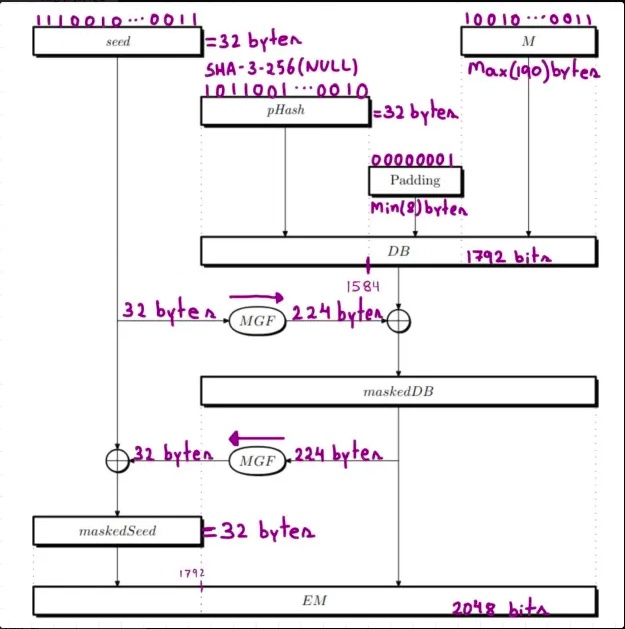
\includegraphics[width=0.8\textwidth]{enc_oaep.png}
    \caption{Diagrama do processo de encapsulamento OAEP}
    \label{fig:enc_oaep}
\end{figure}

\begin{figure}[h]
    \centering
    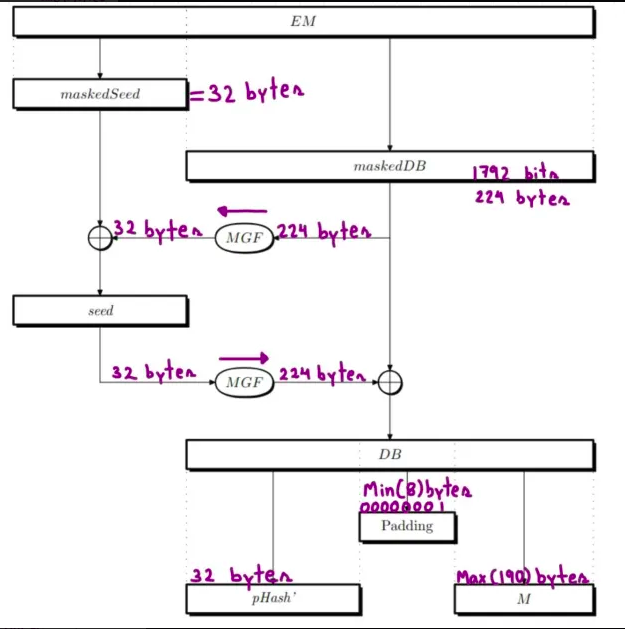
\includegraphics[width=0.8\textwidth]{dec_oaep.png}
    \caption{Diagrama do processo de decapsulamento OAEP}
    \label{fig:dec_oaep}
\end{figure}

\end{document}
